%% =============================================================================
%% SOFTWARE ARCHITECTURE
%% =============================================================================

\section{Software architecture} \label{sec:architecture}

% TODO: Document the crate structure and interfaces

\pkg{prompt2analytics} is organized as a \proglang{Rust} workspace with four crates:

\begin{description}
  \item[\pkg{p2a-core}] Core analytics library implementing all statistical methods
  \item[\pkg{p2a-cli}] Command-line interface (\code{p2a} binary)
  \item[\pkg{p2a-mcp}] Model Context Protocol server (101 tools)
  \item[\pkg{p2a-desktop}] Desktop application with LLM integration
\end{description}

\subsection{Core library}

The core library uses \pkg{polars} \citep{polars} for DataFrame operations,
\pkg{ndarray} \citep{ndarray} for matrix operations, \pkg{faer} \citep{faer}
for linear algebra (Cholesky decomposition, matrix inverse), and \pkg{statrs}
\citep{statrs} for statistical distributions.

\subsection{Interfaces}

% CLI, MCP server, desktop app
Three interfaces provide access to the functionality:
\begin{enumerate}
  \item Command-line interface with hierarchical subcommands
  \item MCP server exposing 101 tools for LLM integration
  \item Desktop application with conversational interface
\end{enumerate}

Figure~\ref{fig:architecture} illustrates the overall software architecture,
showing how the different components interact. The CLI provides direct access
to the analytics engine, while the chat-based interfaces route through an LLM
layer that interprets natural language requests and translates them into
structured tool calls via the MCP protocol.

\begin{figure}[htbp]
\centering
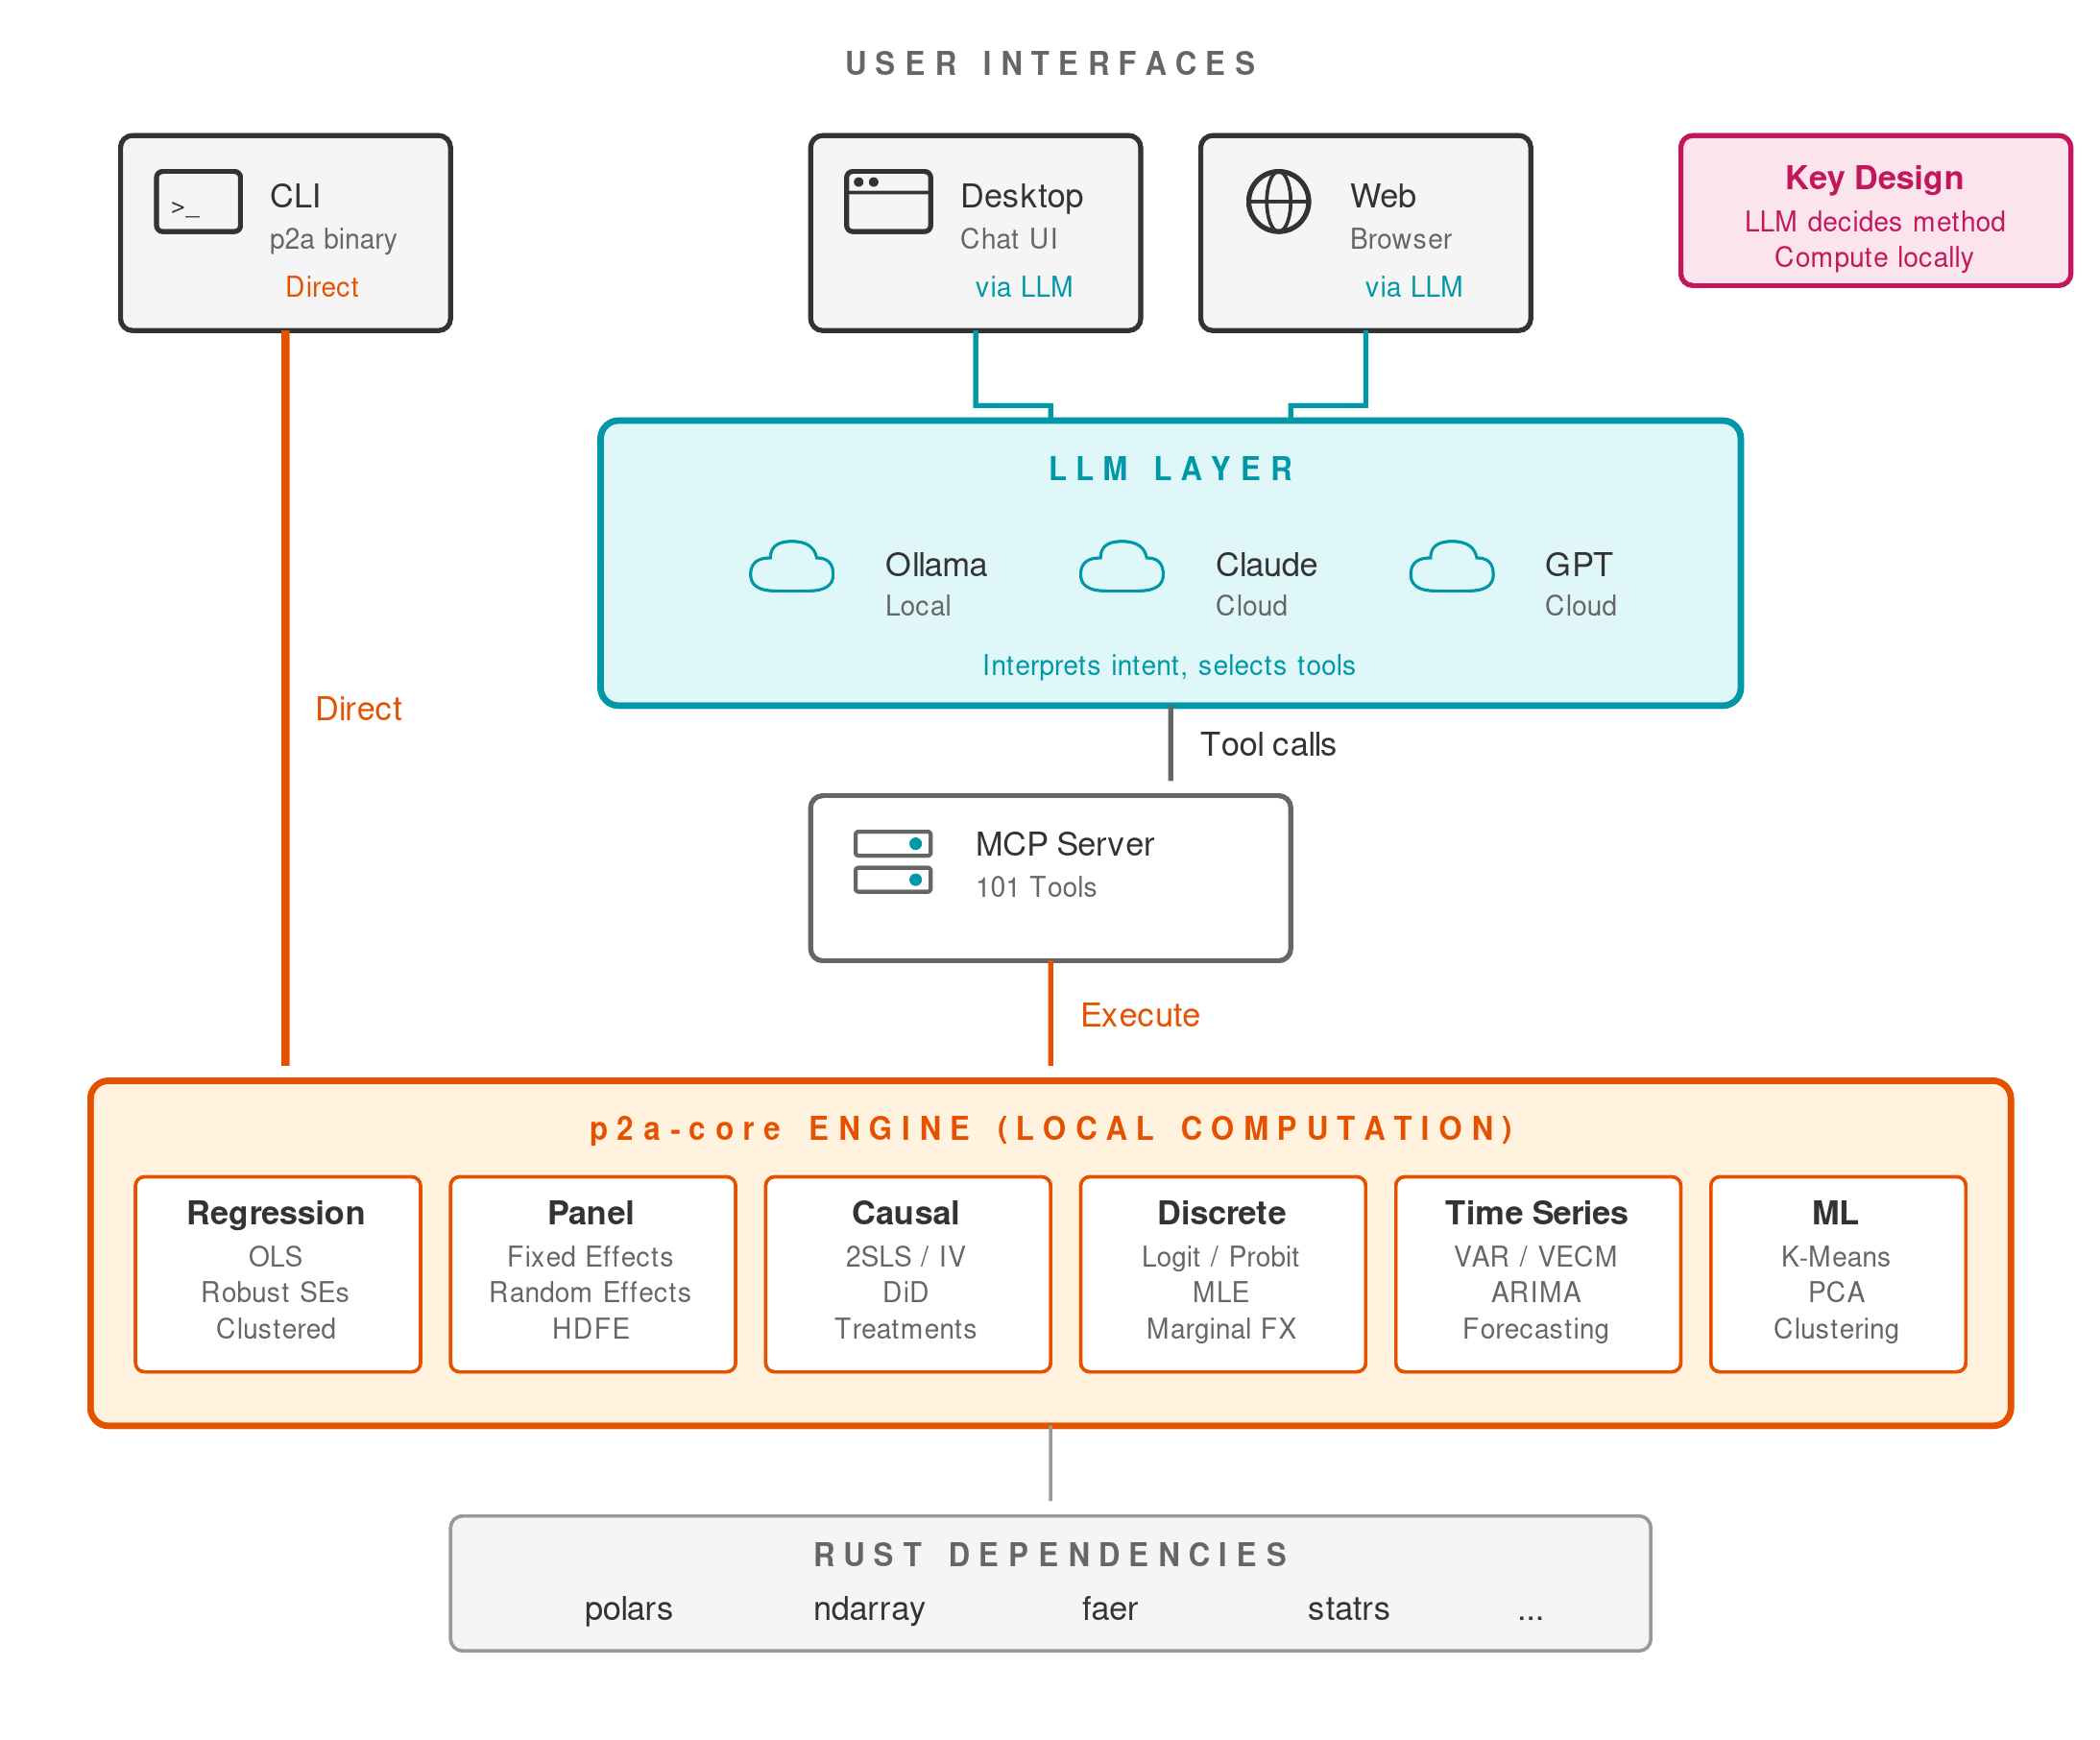
\includegraphics[width=\textwidth]{figures/architecture_v3}
\caption{Software architecture of \pkg{prompt2analytics}. User interfaces
(top) connect either directly to the analytics engine (CLI) or through
LLM providers and the MCP server (chat interfaces). The core analytics
engine implements all statistical methods using pure \proglang{Rust}
dependencies (bottom).}
\label{fig:architecture}
\end{figure}

\subsection{LLM integration via MCP}

The Model Context Protocol (MCP) enables integration with large language
models \citep{MCP:2024}. When a user submits a natural language query through
the chat interface, the LLM interprets the request and generates appropriate
tool calls. Figure~\ref{fig:chat-flow} illustrates this interaction pattern.

\begin{figure}[htbp]
\centering
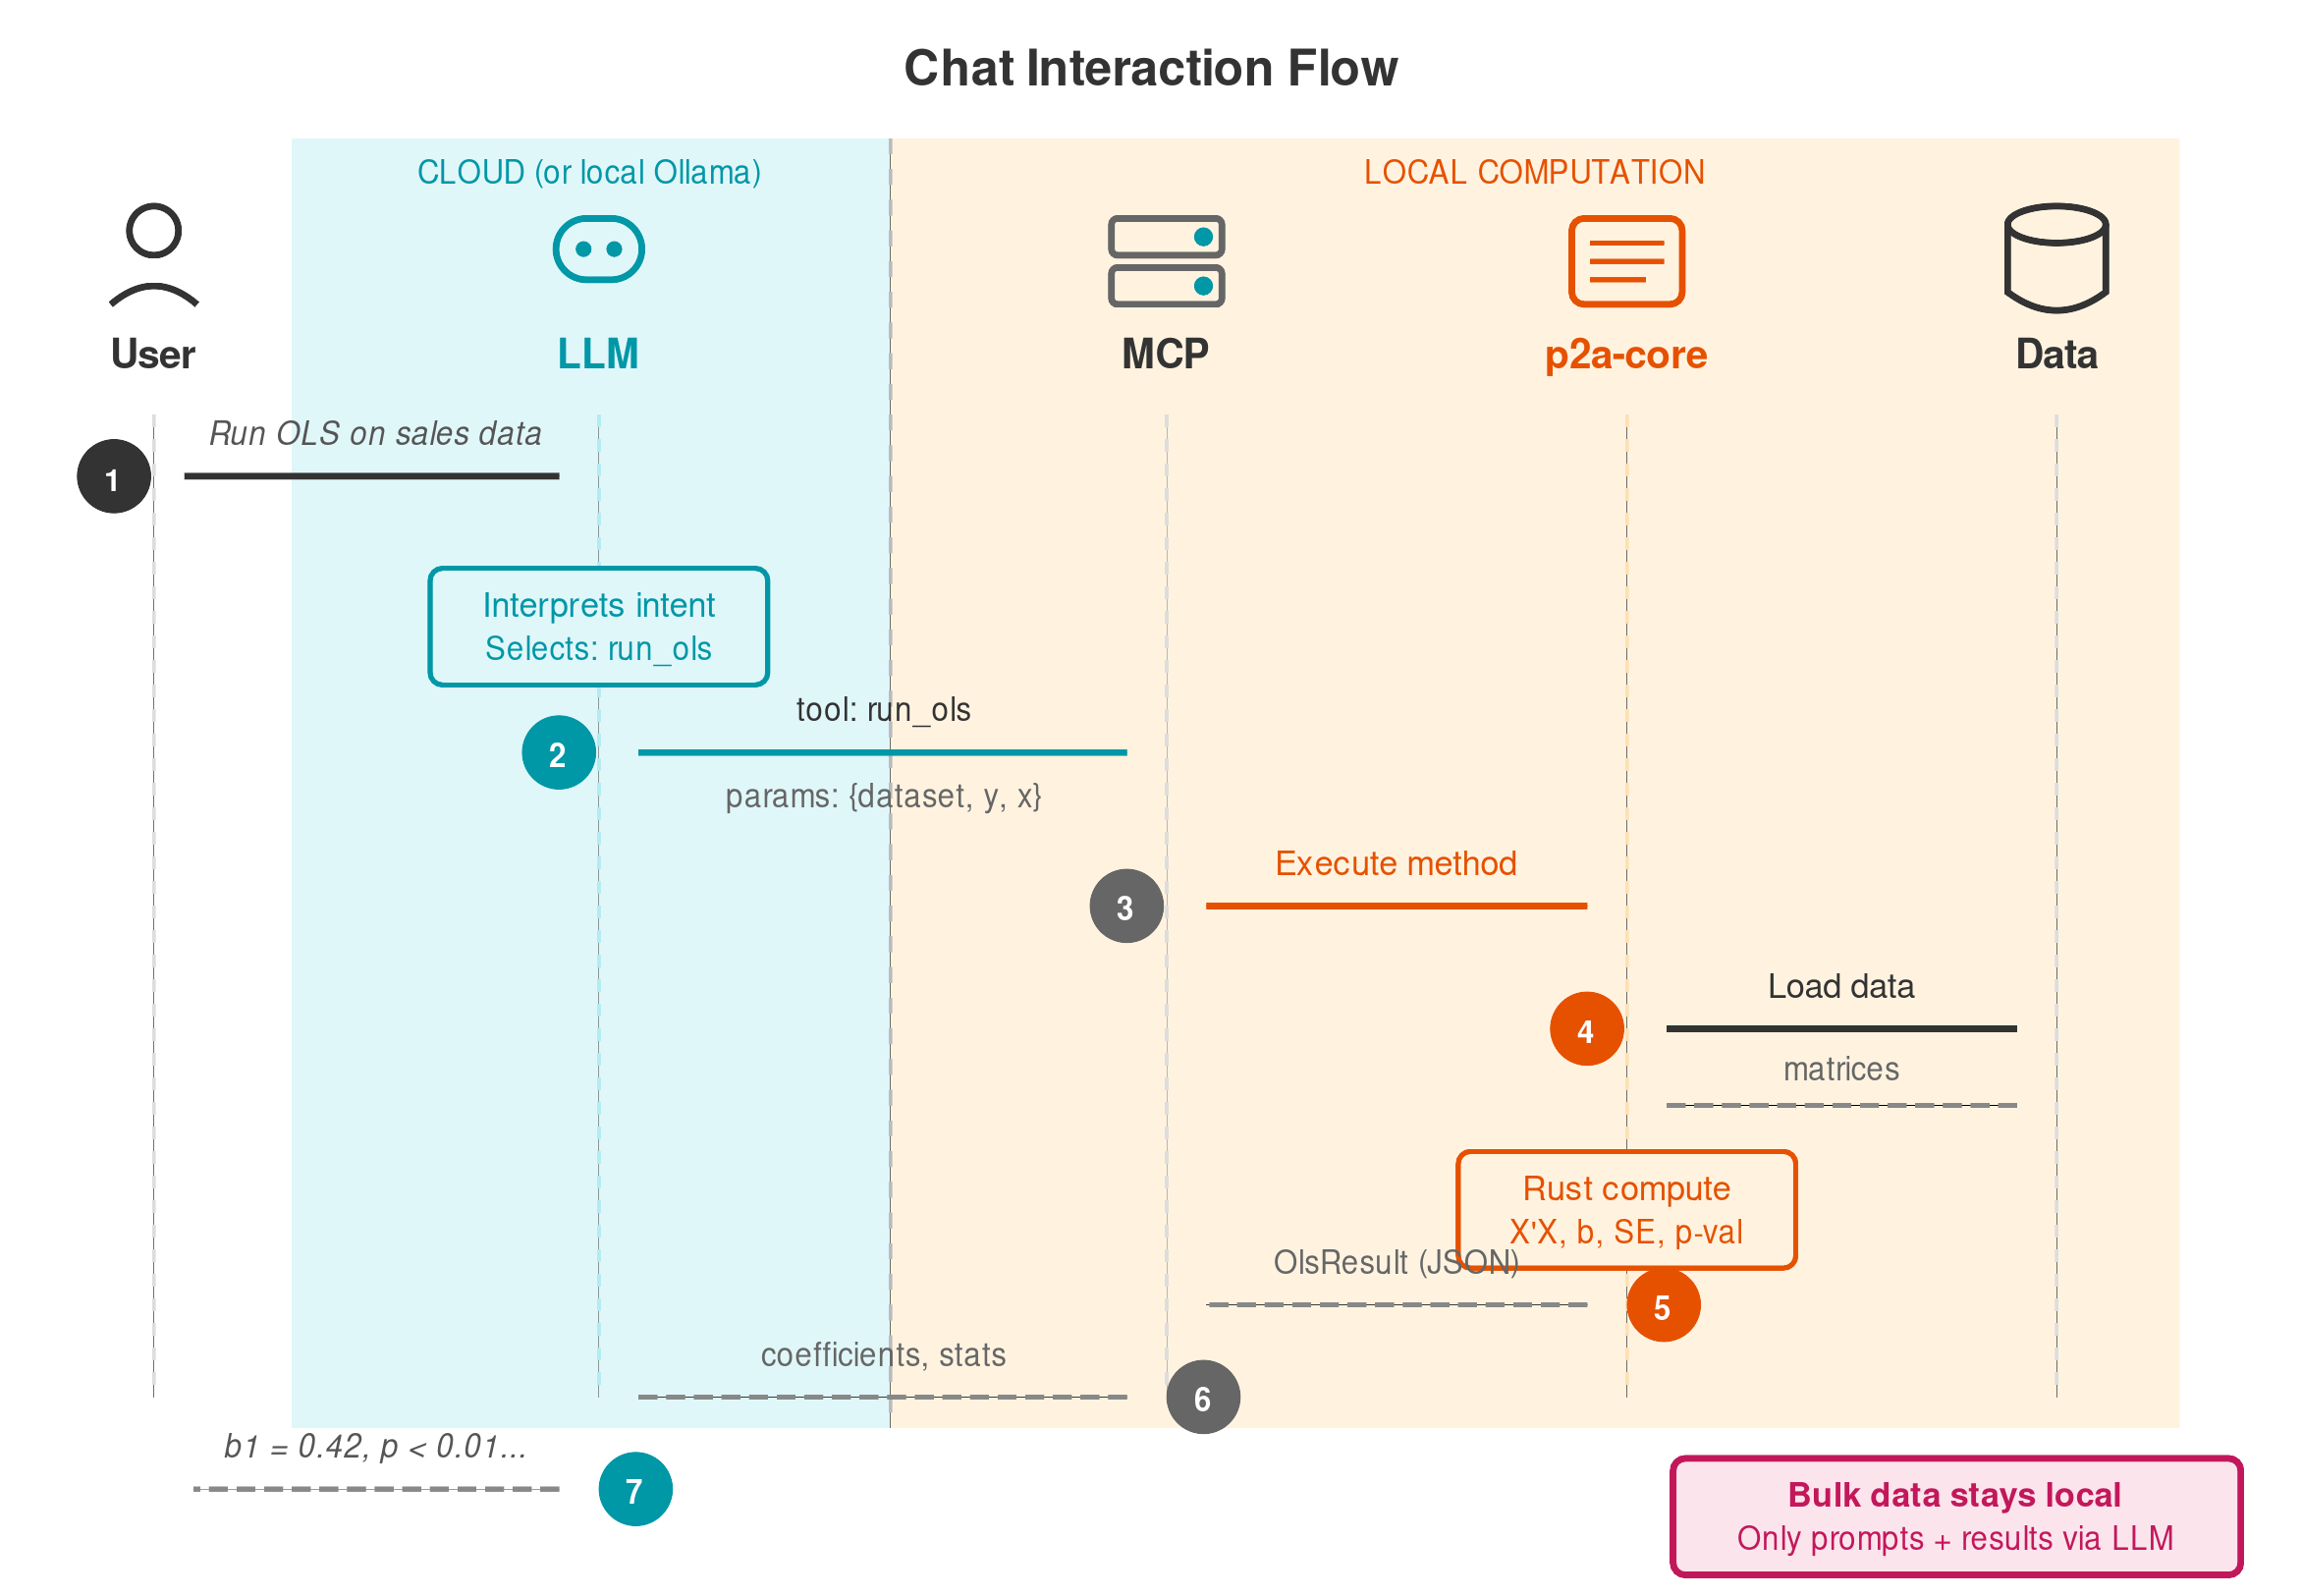
\includegraphics[width=\textwidth]{figures/chat_flow_v2}
\caption{Sequence diagram showing the chat interaction flow. The user's
natural language request (1) is interpreted by the LLM, which generates
a structured tool call (2). The MCP server executes the corresponding
\proglang{Rust} method (3--6), and the result flows back through the
LLM (7--8), which provides a natural language explanation. All data
processing occurs locally; only the prompts and tool parameters are
sent to cloud LLM providers (or processed locally with Ollama).}
\label{fig:chat-flow}
\end{figure}

This architecture ensures that all data processing occurs locally.
The LLM receives tool parameters and requested outputs, but the full dataset
remains on the user's machine. Users should be aware that any explicitly
requested data previews or detailed results will pass through the LLM provider.
For fully local operation, users can deploy Ollama, eliminating any external
data transmission entirely.
